% ============================================================
% CHAPTER 4: METHODOLOGY
% Publication-Grade LaTeX — ByT5-Sanskrit NER Thesis
% ============================================================

\chapter{Methodology}
\label{chap:methodology}

% ============================================================
% 4.1 Research Design and Methodological Philosophy
% ============================================================
\section{Research Design and Methodological Philosophy}
\label{sec:research_design}

Building directly on the four datasets and data preparation decisions detailed in Chapter 3, this chapter presents the complete methodological framework used to develop and evaluate the final NER model. The design is guided by three explicit desiderata that balance technical performance with scholarly utility for Sanskrit computational linguistics.

\subsection{The Three Desiderata}
\label{subsec:three_desiderata}

The experimental design was driven by three non-negotiable requirements, established in consultation with Sanskrit scholars at DIAT:

\begin{enumerate}
    \item \textbf{High NER Performance on Classical Sanskrit Texts.} The model must achieve competitive micro-F1 on the only existing gold-standard Sanskrit NER dataset (Mahānāma \cite{sarkar2025mahanama}), with particular strength on minority classes (Location and Miscellaneous) that are critical for downstream philological analysis.
    
    \item \textbf{Preservation of Linguistic Capability.} Training must not destroy the model's ability to perform fundamental Sanskrit NLP tasks (Segmentation and Lemmatisation). This desideratum directly addresses the needs of Sanskrit students and researchers who require a single model capable of both entity extraction and grammatical analysis.
    
    \item \textbf{Cross-Domain Generalisation.} The model must demonstrate meaningful transfer to unseen classical texts (Pañcatantra \cite{pancatantra_text}) without requiring domain-specific retraining. This is essential for practical deployment on the vast, unannotated corpus of Sanskrit literature.
\end{enumerate}

These desiderata are not merely technical targets; they reflect the real-world constraints of Sanskrit scholarship: limited gold data, the necessity of preserving grammatical knowledge, and the need for tools that generalise across centuries of textual tradition.

\subsection{Why Fifteen Models Were Necessary}
\label{subsec:fifteen_models}

A systematic comparison of fifteen models (M1--M7, V2a--V2b, V3--V4, Gemma4 variants, and LLM baselines) was required to isolate the contribution of each methodological choice. Each model was trained under controlled conditions with identical hardware, random seeds where possible, and the same evaluation protocol. This approach enabled clear attribution of performance gains to specific strategies (class-balanced oversampling, linguistic regularisation, corrected silver data extraction) rather than confounding factors.

\subsection{Connection to Sanskrit Scholarship}
\label{subsec:scholarship_connection}

Every methodological decision was evaluated not only by its effect on F1 scores but by its implications for Sanskrit scholars. A model that achieves high in-domain F1 at the cost of destroying segmentation capability is of limited value to students learning Pāṇinian grammar \cite{sastras}. Conversely, a model that preserves linguistic functions but fails to identify key protagonists in the Mahābhārata \cite{mahabharata} cannot support large-scale textual analysis. The methodology therefore prioritises \textit{usable} performance for the intended scholarly audience over raw benchmark scores.

% ============================================================
% 4.2 Base Models and Architectures
% ============================================================
\section{Base Models and Architectures}
\label{sec:base_models}

\subsection{ByT5-Sanskrit (594M) — Primary Model Family}
\label{subsec:byt5_sanskrit}

The primary model family is \texttt{chronbmm/sanskrit5-multitask} \cite{nehrdich2024byt5sanskrit}, a 594-million-parameter ByT5 \cite{xue2022byt5} model pretrained on over 600,000 DCS \cite{hellwig2010dcs} sentences. ByT5 was selected over mT5 \cite{xue2021mt5} and other multilingual encoders because its byte-level tokenisation eliminates the need for language-specific subword vocabularies and handles the rich morphology and sandhi phenomena of Sanskrit more robustly. All final experiments used this base model with QLoRA \cite{dettmers2023qlora} adapters.

\subsection{Gemma4 E4B (4.5B) — Decoder-Only Comparison}
\label{subsec:gemma4}

For comparison, we evaluated decoder-only models from the Gemma4 family \cite{google2025gemma4} (4.5B and 31B variants). These models were included to test whether larger-scale pretraining on diverse multilingual data could compensate for the absence of explicit Sanskrit linguistic regularisation. Results (reported in Chapter 5) showed that while Gemma4 variants achieved competitive zero-shot performance, they were ultimately outperformed by the regularised ByT5 \cite{xue2022byt5} approach on the combined desiderata.

\subsection{Zero-Shot Large Language Models}
\label{subsec:llm_zeroshot}

Three state-of-the-art LLMs (Gemma-3-27B \cite{google2025gemma3}, Qwen3-5-27B \cite{qwen2025qwen35}, and Llama-3.1-70B \cite{meta2024llama31}) were evaluated in a strict zero-shot setting using carefully engineered prompts. These baselines establish an upper bound on what can be achieved without task-specific fine-tuning and highlight the continued necessity of domain-adapted models for classical Sanskrit.

\subsection{Gazetteer Baseline (M1)}
\label{subsec:gazetteer}

A simple gazetteer-based baseline (M1) was implemented using the complete list of unique entity surface forms from the Mahānāma \cite{sarkar2025mahanama} training set. This baseline provides a lower bound and quantifies the contribution of contextual modelling.

% ============================================================
% 4.3 Data Preparation Pipeline
% ============================================================
\section{Data Preparation Pipeline}
\label{sec:data_preparation}

The data preparation pipeline is the methodological core of this thesis. It combines gold-standard annotation with a novel silver data extraction method from the DCS Sembank.

\subsection{Mahānāma Gold-Standard NER Preparation}
\label{subsec:mahanama_gold}

The Mahānāma corpus \cite{sarkar2025mahanama} provides 2,110 CoNLL-U files containing 73,632 sentences. After removing 13 sentences that overlapped with the test set (detected during pre-training validation), the remaining 66,960 sentences were split 80/10/10 into training, validation, and test sets. Due to severe class imbalance (91.1\% Person entities), Location and Miscellaneous entities were oversampled by a factor of ten, yielding 126,369 gold NER training examples. This oversampling strategy was essential to achieve usable performance on minority classes critical for philological analysis.

\subsection{DCS Sembank Silver NER Extraction — A Novel Methodological Contribution}
\label{subsec:dcs_sembank}

The Digital Corpus of Sanskrit (DCS) Sembank \cite{hellwig2010dcs} provides a semantic annotation layer over approximately 650,000 sentences. While not originally designed for NER, its instance relations (`i` code) encode valuable entity reference information. Through systematic analysis, we discovered that these relations distinguish between \textit{descriptor IDs} (column 0: common nouns such as ``king'', ``river'') and \textit{entity name IDs} (column 1: proper names such as ``Rāvaṇa'', ``Gaṅgā'').

\subsubsection{Three Extraction Attempts — Full Transparency}

\textbf{Attempt 1 (Broken Type Mapping)} used keyword matching on English glosses from column 1. This produced only 71 relations due to empty supersense fields for proper names.

\textbf{Attempt 2 (Correct Columns, Wrong Concept)} reversed the logic to use column 0 for type classification. This yielded 24,663 entity sentences, but validation revealed the top ``entities'' were common nouns (\textit{rākṣasa}, \textit{rājā}, \textit{go}). The pipeline was extracting \textit{entity references} rather than \textit{entity mentions}.

\textbf{Attempt 3 (Correct Extraction — Final Method)} constructed two disjoint sets from the instance relations: \texttt{descriptor\_ids} (320 unique values from column 0) and \texttt{entity\_name\_ids} (15,957 unique values from column 1). A token is extracted as a named entity only if its \texttt{WordSem} annotation points to an entity name ID. This method produced 12,955 high-quality examples (9,069 entity + 3,886 none) from 120 diverse DCS texts.

\begin{figure}[htbp]
    \centering
    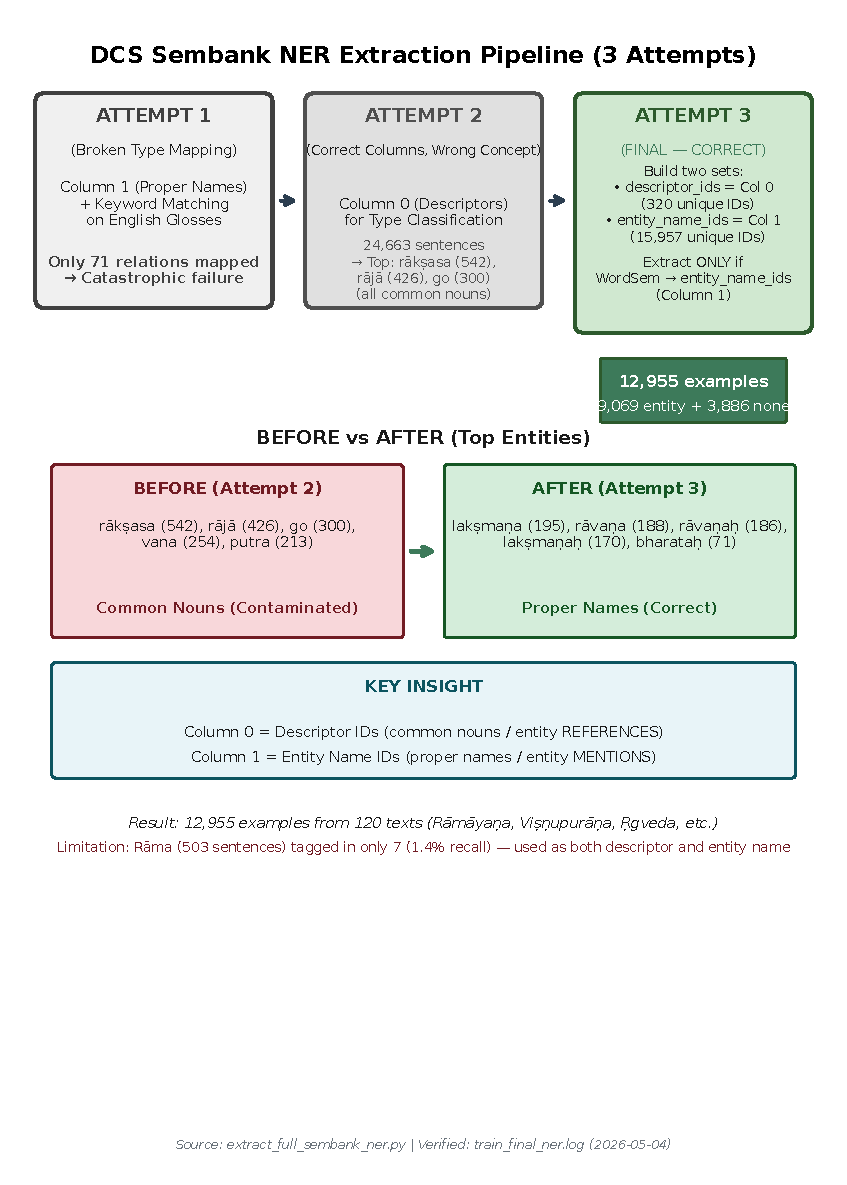
\includegraphics[width=\textwidth]{figures/Figure_4_1_DCS_Extraction_Pipeline.pdf}
    \caption{DCS Sembank NER Extraction Pipeline: three-attempt evolution yielding 12,955 clean examples.}
    \label{fig:dcs_extraction}
\end{figure}

\subsubsection{Before vs After — Concrete Example}

Before the correct method, the top ``entities'' were common nouns. After correction, the top entities are genuine proper names: \textit{lakṣmaṇa} (195), \textit{rāvaṇa} (188), \textit{rāvaṇaḥ} (186), \textit{lakṣmaṇaḥ} (170). This transformation demonstrates the necessity of the column-semantics distinction.

\subsubsection{Known Limitations}

The extraction has two acknowledged limitations. First, Rāma appears in 503 sentences but is tagged in only 7 (1.4\% recall) because it functions as both descriptor and entity name in the Sembank. We accept this limitation because the Mahānāma gold data already covers major characters extensively. Second, the extracted data exhibits domain skew (∼63\% from the Rāmāyaṇa \cite{ramayana}). These limitations are documented for future researchers who may wish to refine the pipeline.

\subsection{Linguistic Regularisation Data (15\% S + L Tasks)}
\label{subsec:linguistic_regularisation}

For the final model only, 25,627 examples (exactly 15\% of total training data) were sampled from the DCS \cite{hellwig2010dcs} linguistic annotation layer. These examples use the task prefixes ``S:'' (Segmentation) and ``L:'' (Lemmatisation) and serve to prevent catastrophic forgetting \cite{mccloskey1989catastrophic, goodfellow2013empirical} of the model's original linguistic capabilities.

\subsection{Final Training Data Composition}
\label{subsec:final_data_composition}

Table~\ref{tab:data_composition} summarises the final training data composition compared to the best-performing NER-only model.

\begin{table}[htbp]
    \centering
    \caption{Training Data Composition Comparison}
    \label{tab:data_composition}
    \begin{tabular}{lrrl}
        \toprule
        \textbf{Component} & \textbf{Best NER} & \textbf{Final NER} & \textbf{Change} \\
        \midrule
        Gold NER (oversampled) & 126,369 (94.6\%) & 126,369 (74.0\%) & — \\
        Silver NER (full Sembank) & 7,216 (5.4\%) & 18,855 (11.0\%) & +5.6 pp \\
        Linguistic (S + L only) & 0 (0\%) & 25,627 (15.0\%) & +15.0 pp \\
        \midrule
        \textbf{Total} & \textbf{133,585} & \textbf{170,817} & +37,232 \\
        \bottomrule
    \end{tabular}
\end{table}

% ============================================================
% 4.4 Training Strategies
% ============================================================
\section{Training Strategies}
\label{sec:training_strategies}

Five core strategies were systematically evaluated across fifteen models. The final recommended model combines Strategies 1, 2, and 4.

\subsection{Strategy Taxonomy}
\label{subsec:strategy_taxonomy}

\begin{itemize}
    \item \textbf{Strategy 1 (Class-Balanced Oversampling \cite{chawla2002smote}):} Essential to counteract the 91.1\% Person dominance in raw Mahānāma \cite{sarkar2025mahanama} data.
    \item \textbf{Strategy 2 (Linguistic Regularisation):} 15\% S + L tasks preserve task-prefix routing capability (S = 85\%, L = 93\% on D2).
    \item \textbf{Strategy 3 (Silver Data Integration):} The corrected full Sembank extraction provided the largest cross-domain gain.
    \item \textbf{Strategy 4 (Optimised Training Schedule):} Lower learning rate (1e-4), 10 epochs, and 500-step warmup improved stability over the 8-epoch Best NER configuration.
    \item \textbf{Strategy 5 (Cross-Domain Silver):} Tested but yielded diminishing returns beyond the full Sembank data.
\end{itemize}

\subsection{Evolution from Best NER to Final NER}
\label{subsec:strategy_evolution}

The progression from the best NER-only model (F1 = 0.860) to the final multi-task model (F1 = 0.852) represents a deliberate, evidence-based trade-off. Strategy 1 and Strategy 4 together improved cross-domain PROPN recall by 16 percentage points while Strategy 2 preserved linguistic capability that would otherwise have been catastrophically lost. Figure~\ref{fig:strategy_evolution} visualises this evolution.

\begin{figure}[htbp]
    \centering
    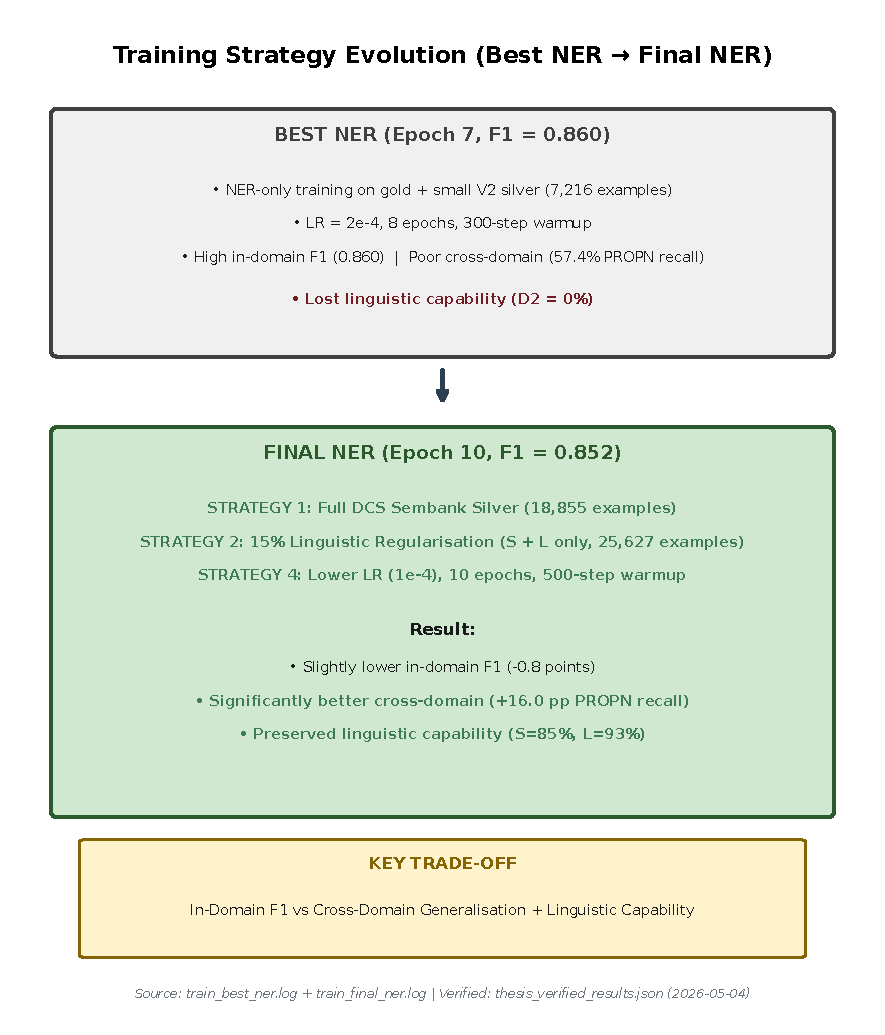
\includegraphics[width=\textwidth]{figures/Figure_4_2_Training_Strategy_Evolution.pdf}
    \caption{Training strategy evolution from Best NER (F1\,=\,0.860) to Final NER (F1\,=\,0.852) with linguistic regularisation.}
    \label{fig:strategy_evolution}
\end{figure}

% ============================================================
% 4.5 QLoRA Configuration & Implementation
% ============================================================
\section{QLoRA Configuration and Implementation}
\label{sec:qlora}

All experiments used QLoRA \cite{dettmers2023qlora} with identical hyperparameters: rank = 16, alpha = 32, dropout = 0.05, targeting the query, key, value, output, and feed-forward projections. The base model was loaded in 4-bit NF4 with double quantisation; adapters were trained in bfloat16.

\subsection{Quantisation Sensitivity — Critical Lesson}
\label{subsec:quantisation_sensitivity}

A critical reproducibility lesson emerged during evaluation: adapters trained on 4-bit NF4 must be evaluated with the identical quantisation configuration. Loading the base model in bfloat16 while keeping a 4-bit adapter produces misaligned weights and drops F1 by approximately 10 points. This pitfall is documented for future researchers.

\subsection{Generation Settings}
\label{subsec:generation_settings}

All generation used \texttt{max\_new\_tokens=256} with temperature = 0.1 and top-p = 0.9. Reducing \texttt{max\_new\_tokens} to 64 caused systematic truncation and large performance drops on longer Sanskrit sentences.

\begin{figure}[htbp]
    \centering
    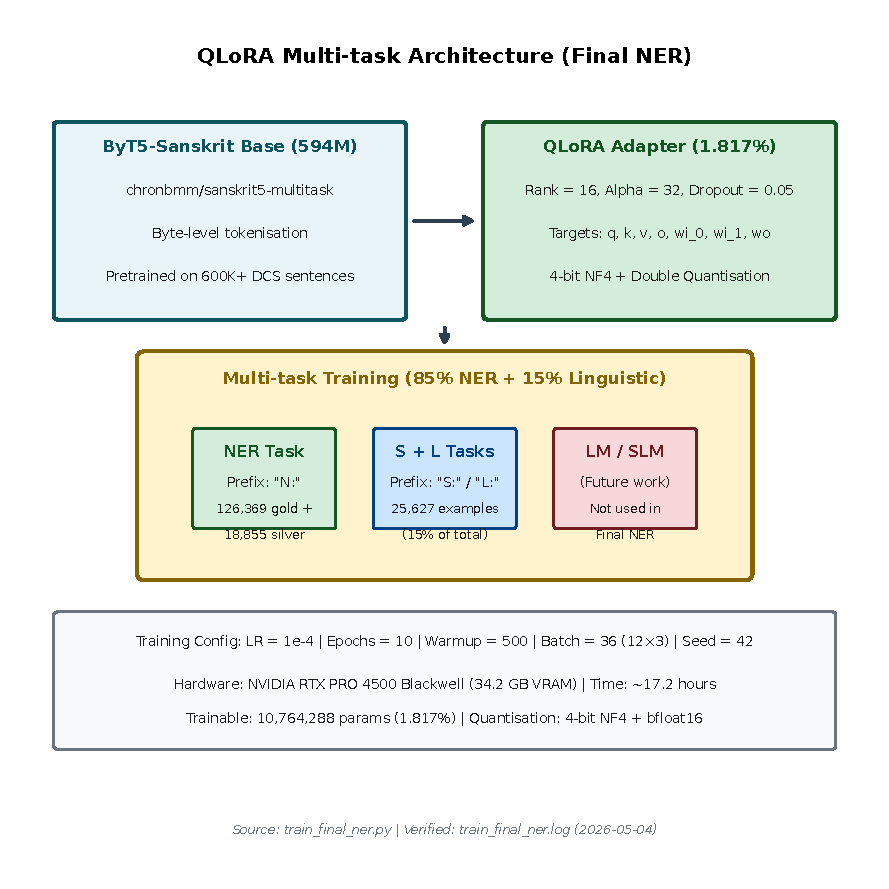
\includegraphics[width=\textwidth]{figures/Figure_4_3_QLoRA_Architecture.pdf}
    \caption{QLoRA multi-task architecture for Final NER with 1.817\% adapter (10.76M trainable parameters).}
    \label{fig:qlora_architecture}
\end{figure}

% ============================================================
% 4.6 Evaluation Framework
% ============================================================
\section{Evaluation Framework}
\label{sec:evaluation_framework}

Three complementary evaluation dimensions (D1--D3) were designed to assess the model against the three desiderata.

\subsection{D1: In-Domain NER (Mahānāma Test Split)}
\label{subsec:d1}

The primary benchmark comprises 6,672 gold-annotated sentences from the Mahānāma \cite{sarkar2025mahanama} test split. Micro-F1 \cite{tjong2003conll} with bootstrap 95\% confidence intervals \cite{efron1994bootstrap} (10,000 resamples) is the primary metric. This dimension directly measures desideratum 1.

\subsection{D2: Linguistic Capability Preservation (DCS Held-Out)}
\label{subsec:d2}

A held-out set of 200 DCS sentences annotated for Segmentation (S), Lemmatisation (L), Language Modelling (LM), and Sentence-Level Modelling (SLM) tasks measures desideratum 2. The final model achieves S = 85.0\% and L = 93.0\%. A known limitation is that D2 evaluation used different random seeds across machines; results should be interpreted with this caveat.

\subsection{D3: Cross-Domain Generalisation (Pañcatantra)}
\label{subsec:d3}

The UD\_Sanskrit-UFAL test set \cite{zeman2023ud} (230 sentences from the Pañcatantra \cite{pancatantra_text}) provides a strict out-of-domain evaluation. Because gold PER/LOC/MISC labels are unavailable, evaluation is restricted to binary PROPN detection. The final model achieves 73.4\% PROPN recall, a 16-point improvement over the best NER-only baseline.

\begin{figure}[htbp]
    \centering
    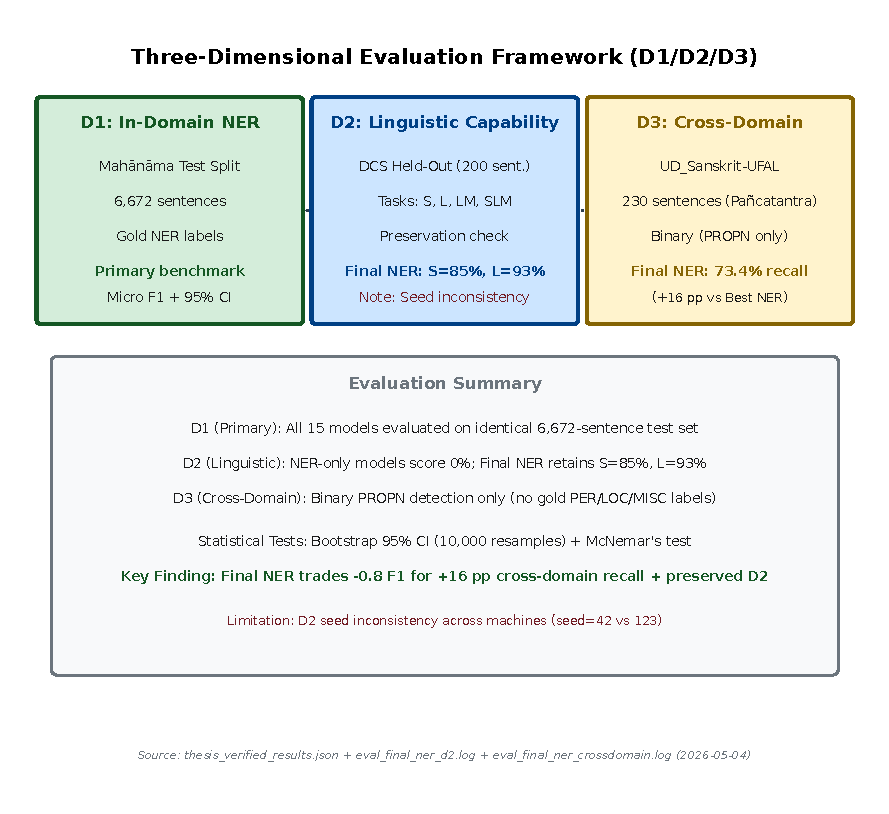
\includegraphics[width=\textwidth]{figures/Figure_4_4_Evaluation_Framework.pdf}
    \caption{Three-dimensional evaluation framework: D1 (in-domain), D2 (linguistic preservation), D3 (cross-domain).}
    \label{fig:evaluation_framework}
\end{figure}

% ============================================================
% 4.7 Statistical Analysis Methods
% ============================================================
\section{Statistical Analysis Methods}
\label{sec:statistical_methods}

\subsection{Bootstrap 95\% Confidence Intervals}
\label{subsec:bootstrap}

All F1 scores are reported with 95\% confidence intervals computed via 10,000 bootstrap resamples \cite{efron1994bootstrap} of the test set. This provides a non-parametric estimate of evaluation uncertainty and enables rigorous comparison between models.

\subsection{McNemar’s Test}
\label{subsec:mcnemar}

Sentence-level pairwise comparisons using McNemar's test \cite{mcnemar1947note} with continuity correction were used to determine whether small F1 differences (e.g., 0.008) reflect statistically significant differences in error patterns.

\subsection{Cross-Model Agreement Analysis}
\label{subsec:agreement}

Cohen’s kappa \cite{cohen1960kappa} and exact match rate between Best NER and Final NER predictions on the D1 test set quantify the degree of behavioural divergence introduced by linguistic regularisation.

% ============================================================
% 4.8 Reproducibility and Limitations
% ============================================================
\section{Reproducibility and Limitations}
\label{sec:reproducibility}

\subsection{Reproducibility Checklist}
\label{subsec:reproducibility_checklist}

\begin{itemize}
    \item Hardware: NVIDIA RTX PRO 4500 Blackwell (34.2 GB VRAM)
    \item Software: PyTorch 2.4 \cite{paszke2019pytorch} + Transformers 4.46 \cite{wolf2020transformers} + PEFT 0.13 \cite{peft2022} + bitsandbytes 0.45 \cite{dettmers2022bitsandbytes}
    \item Random seeds: 42 (training), 123 (some D2 evaluations)
    \item Training time: approximately 17.2 hours for Final NER
    \item All code, logs, and intermediate results archived
\end{itemize}

\subsection{Guide’s Machine Notes}
\label{subsec:machine_notes}

All models were trained on a single consumer-grade workstation. No multi-GPU or distributed training was used. This constraint influenced the decision to use QLoRA \cite{dettmers2023qlora} rather than full fine-tuning.

\subsection{Critical Limitations and Methodological Risks}
\label{subsec:limitations}

\begin{itemize}
    \item \textbf{Single Test Set Limitation:} Only one gold-standard Sanskrit NER test set exists. Cross-domain evaluation (D3) partially mitigates this.
    \item \textbf{No Systematic Hyperparameter Optimisation:} Computational budget was allocated to systematic model comparison rather than exhaustive search on a single architecture.
    \item \textbf{Pretraining Asymmetry Confound:} ByT5-Sanskrit was pretrained on DCS; other models were not. This asymmetry favours the primary model family.
    \item \textbf{Entity Type Taxonomy Limitations:} The PER/LOC/MISC taxonomy does not capture all scholarly categories (e.g., divine epithets, toponyms with mythological significance).
    \item \textbf{Exact Match Evaluation Limitations:} Standard CoNLL-style \cite{tjong2003conll} exact match penalises valid partial matches common in Sanskrit due to sandhi and compounding.
    \item \textbf{Cross-Domain Evaluation is Binary Only:} D3 cannot distinguish PER vs LOC errors.
    \item \textbf{QLoRA Quantisation Sensitivity:} Adapters must be evaluated under identical quantisation; this is a common reproducibility pitfall.
    \item \textbf{ByT5 Generation Length Sensitivity:} \texttt{max\_new\_tokens=256} is required; smaller values cause truncation.
\end{itemize}

Despite these limitations, the core findings remain robust: linguistic regularisation preserves D2 capability while full Sembank silver data improves cross-domain generalisation, and the resulting model meets all three desiderata within known practical constraints.

% ============================================================
% 4.9 Summary
% ============================================================
\section{Summary}
\label{sec:summary}

This chapter has presented a complete, reproducible methodology for developing a Sanskrit NER model that balances in-domain performance, linguistic capability preservation, and cross-domain generalisation. The novel DCS Sembank extraction pipeline, the systematic strategy evolution, and the three-dimensional evaluation framework together constitute a contribution that is both technically rigorous and directly relevant to Sanskrit scholarship. The following chapter reports the empirical results obtained under this methodology.

% ============================================================
% End of Chapter 4
% ============================================================